\documentclass[tikz,border=6pt]{standalone}
\usepackage{amsmath,amssymb}
\usetikzlibrary{arrows.meta,calc}
\begin{document}
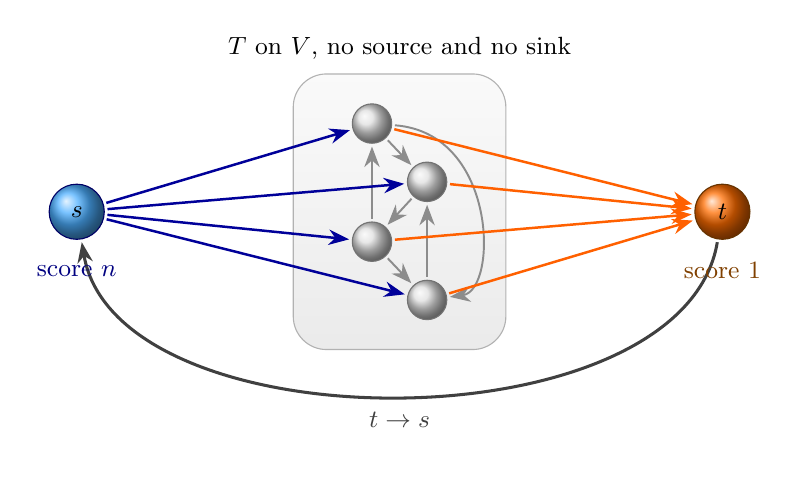
\begin{tikzpicture}[>={Stealth[length=2.6mm]},
  old/.style={circle,shading=ball,ball color=gray!25,draw=black!55,minimum size=5mm,inner sep=0pt},
  sv/.style={circle,shading=ball,ball color=blue!45!cyan!70,draw=blue!40!black,minimum size=7mm,inner sep=0pt,font=\small},
  tv/.style={circle,shading=ball,ball color=orange!85!red,draw=orange!40!black,minimum size=7mm,inner sep=0pt,font=\small},
  sa/.style={->,draw=blue!60!black,line width=0.9pt,shorten >=1pt,shorten <=1pt},
  ta/.style={->,draw=orange!75!red,line width=0.9pt,shorten >=1pt,shorten <=1pt},
  ia/.style={->,draw=black!45,line width=0.7pt,shorten >=1pt,shorten <=1pt}]
  % the old tournament T, drawn as a shaded panel
  \shade[rounded corners=12pt,top color=gray!4,bottom color=gray!16,draw=gray!60] (-1.35,-1.75) rectangle (1.35,1.75);
  \node[font=\small] at (0,2.08) {$T$ on $V$, no source and no sink};
  \node[old] (a) at (-0.35,1.12) {};
  \node[old] (b) at (0.35,0.38) {};
  \node[old] (c) at (-0.35,-0.38) {};
  \node[old] (d) at (0.35,-1.12) {};
  \draw[ia] (a) -- (b); \draw[ia] (b) -- (c); \draw[ia] (c) -- (d);
  \draw[ia] (c) -- (a); \draw[ia] (d) -- (b);
  \draw[ia] (a) .. controls (1.25,1.0) and (1.25,-1.0) .. (d);
  \node[sv] (s) at (-4.1,0) {$s$};
  \node[tv] (t) at (4.1,0) {$t$};
  \foreach \x in {a,b,c,d} \draw[sa] (s) -- (\x);
  \foreach \x in {a,b,c,d} \draw[ta] (\x) -- (t);
  \draw[->,line width=1.1pt,black!75,shorten >=1pt,shorten <=1pt] (t) .. controls (3.6,-3.0) and (-3.6,-3.0) .. node[pos=0.5,below=2pt,font=\small] {$t\to s$} (s);
  \node[font=\small,blue!50!black] at (-4.1,-0.75) {score $n$};
  \node[font=\small,orange!50!black] at (4.1,-0.75) {score $1$};
\end{tikzpicture}
\end{document}
